\documentclass{scrartcl}
\usepackage{fullpage}
\usepackage{pdfpages}
\usepackage{graphicx}

\setlength{\parindent}{0.0in}
\setlength{\parskip}{0.1in}

\addtolength{\topmargin}{-1cm}
\addtolength{\textheight}{2cm}
\addtolength{\hoffset}{-0.5cm}
\addtolength{\textwidth}{1cm}

\title{Human-Centred Design}
\subtitle{CALMist - The Elimination of Stress in our Day to Day Living}
\author{Christopher Bowles, Jack Bracewell, Craig Ellis,\\David Harrison, Karl Kelly, Milan Misak, Daniel Randall}
\date{}

\begin{document}
\maketitle
\tableofcontents
\clearpage

\section{Abstract}
Stress is a common factor in people's lives. It affects their ability to work and play, and can have serious health
implications, especially if left unchecked. Interviewing a number of employees of certain firms, it is clear that
people want a solution, but are not always aware when it is that they are most stressed. We propose a couple of
wearable devices that measure stress throughout the day, with a gamified companion website to provide feedback,
stress-reducing tips and encouragement.

\section{Problem Statement}
Personal well-being and happiness is a priority for everyone.
Stress is one of the leading causes of illness and depression in the country.
In order to provide a solution to provide a high quality service at a minimal cost,
we need to produce an unobtrusive user friendly product to improve quality of life.

\section{The Impact of Stress}
Stress is the adverse reaction people have to excessive pressures or other types of demand placed on them.
It is one of the leading causes for health issues in the modern world, and has implications for
employees, employers and the health system.

For employees, a study showed that 75\% of illnesses that required the employee to take time off work were
the direct result of stress. Coupled with the fact that people sufferring from excessive stress spend around 50\%
more on medical expenses in America, we can see that this puts an enormous strain on health services, especially
if we consider countries like the UK, where the figure is probably similar but the health system is publicly funded.
Surprisingly, another study shows that only about 40\% of people in the UK describe their job as stressful. However,
given the number of complaints we heard during the interview process, we question this figure.

For employers, the obvious problem is that they are losing work (as employees take stress-related sick leave) and thus
potentially money. To put this in perspective, in the 2009/10 business year, an estimated 9.8 million working days
were lost in the UK due to work-related stress. This puts stress-related sick leave above strokes, heart attacks and
cancer as a cause of extended workplace absence. It isn't much of a stretch of the imagination to reckon that this
probably results in something of a vicious cycle. People are stressed at work so they need sick leave. Less work gets
done because so many people are taking stress-related sick leave. When they get back, looming deadlines mean more work
in a shorter amount of time, which leads to more stress, and thus more health issues and sick leave, and so on and so forth.

\section{Interviews Process}
When we identified our problem we needed to be able to create a realistic persona
in order to develop for. To this end we needed to find out about real people
who have experienced stress. To facilitate this we decided that we should
develop questionaires and go out and talk to people about stress and get them to 
fill this out. A lot of people talked to us but didn't want to fill out the 
questionaire.

In the appendix I have included a few of the responses we got. 

\section{Interview Results}
The interviews suprised us a lot. From it we realised that stress
affected many more people than what you would expect. For example, 
one of the people we interviewed revealed to us that he actually
had a psychologist to help him deal with his stress. This was
suprising considering the job the person had, a clerk at Ryman.
This isn't a job which would normally be considered high stress
however this person needed to get a psychologist to help him cope.

Another person we interviewed worked at Kodak, his responses were 
equally surprising. At the start of his day he spent about two hours
doing stress management activities such as yoga and breathing exercises.
He also had attended seminars about coping with stress.

We interviewed a library assisstant as well at one point. She 
herself didn't suffer too badly from stress throughout the day
but she did tell us that the most stressful time of day for her was
actually travelling to and from work. This was interesting as
none of us had considered that travelling was a trigger for stress.
We brought this up with other people we interviewed and they told
us that travelling was very stressful for them as well. The
interesting thing though is that they themselves hadn't realised
that travelling was stressing them out until they were asked by
us.

The main things we took from this was that stress affected much
more people than most people realise and that even if you aren't
in a high stress job, your job can be very stressful. Also 
quite a lot of people don't even realise what it is that stresses
them unless it's pointed out to them. This information was used
in both the design of our persona, Lydia, and in the development 
of the solution.

\section{Our Persona - Lydia}
We saw from the interviews that many people find travelling and dealing with customers to be the most stressful parts of their day.
Therefore, we focused on a persona that had to deal with these problems regularly - Lydia. She is 53 years old, and works at Ryman
(and often has to deal with awkward customers). She has 2 children, and must collect them both from school every day after work.
Lydia travels to work by tube every day, and collects her children from school by car. Even though she has all the attributes that
should make her extremely stressed, she is not all that extraordinary; she is somebody that you might expect to see every day. This
reinforces the fact that stress affects everyone - it is a problem that really needs to be solved.

\section{Development of our Idea}
After interviewing people and developing the persona we were going to focus on, we decided we were ready to try and come up with
a solution. In total, we came up with 2 ideas that we eventually rejected, and combined what we felt were the best elements
of the two into our final solution.

\subsection{Idea 1 - Self Help Website}
Our first idea was what can only be described as a self-help website. Users would log on to read tips, and we would attempt to
design everything around the idea of calm (so using light blue and/or green colours, as they are commonly deemed relaxing,
and gentle wording). The website would also have a user forum, so people can talk to others about their problems and advise
other people (something that in itself can be quite calming).

However, although this sounds like a decent solution on paper, we saw a number of problems with it.
For a start, it does not take the user's emotional needs into account. Stress is a very personal thing, and people do not
tend to want to talk about it. Indeed, we found we were very often turned down when trying to interview people during the
interview stage. It's true that the internet allows for a certain anonymity, and sometimes it's actually easier to talk
about personal things with complete strangers, but there's still always going to be that sense of taboo about talking about
such things, as well as the feeling of vulnerability the users will likely feel by opening up. As such, we don't think users
are that likely to actually open up, which means the forum would not be used to its full potential. Indeed it may actually
discourage the potential user from using the service at all, despite the forum being optional. Stress is a very delicate
topic, and this idea just isn't sensitive enough.

Furthermore, except for the
forum element, it's not particularly interactive. It's essentially just an online book. Yes, things could be added to it, and we
could implement features such as ``tip of the day'', but it's still passively reading about stress avoidance. This may well be
enough for some people, but we doubt it would be for most. It in no way encourages people through the more stressful times or
motivates them to improve themselves. What would be needed is some way of making it more active and engaging. The obvious
solution would be gamification. However, we're not really sure how you can gamify this. A point for every tip you read?
That would just turn it into a study game, and in no way measure actual progress or give any indication of how stressed the user
is/is not. The system needs to actively measure the user's progress to provide the needed level of interaction. This lead
us on to our second idea.

\subsection{Idea 2 - Stress Alerts}
Our second idea was some form of a wearable device, such as a bracelet. It would be constantly measuring your stress levels.
Research shows that skin conductance varies with stress, along with breathing pattern. As such, this device would measure
skin conductance. The idea is that it would have a mini alarm, and alert you when your stress levels become ``too high''
(a subjective property, so of course some calibration would probably be required).

This certainly does solve the problem of lack of quantification present in the previous idea, so we didn't want to drop
the idea entirely. However, there is one very big and obvious problem. This, too, isn't sensitive enough to the user's
delicate state, but rather than being too passive like the first idea, it's far too agressive.

Consider someone who is currently in a period of high stress. Perhaps they've just been fired, or perhaps a subordinate has
done something incorrectly and caused them a lot more work. If you're fired, you probably need a short period of ``grief''
to get back on your feet, and yes, if someone has messed up, getting stressed about it is unproductive. But now imagine what
affect adding a device saying ``you are stressed'' would have.

When people are stressed, they don't want to be told they are stressed. They may want any manner of thing, but awareness
is seldom one of them. Hence, having an alarm that goes off when they are stressed is likely to just make them even more
stressed. It would make a bad situation worse. Hence, this idea in its present form was quickly rejected. The method of
measurement and quantification did, however, go on to form the backbone of our final idea.

\subsection{Final Idea}

As we learnt from research into our second idea, stress can be quantified by measuring skin conductance and breathing pattern.
The user needs to be given feedback based upon actual real-world measurements, but it's counter-productive to do this in
real-time. Hence, for our final idea, we proposed maintaining the idea of constant measurement for analysis,
but completely abandoning the idea of real-time feedback, instead opting for end-of-the-day at-the-user's-leisure feedback.

What we mean by this is that we still have a device that measures stress through skin conductance.
These measurements will be somehow uploaded
to a computer (details of implementation are in following sections). The computer would then let the user view a simplified version
of the readings to see how their stress levels varied throughout the day. This would also, obviously, let them see when
they were most stressed, and trivially but worth a mention, low stress.

It's true that people don't always know what exact circumstances cause them to be stress, but with so much emphasis on the
negative, people seem to even more often not know what causes them to be calm. With the ability to review stress levels throughout
the day, the user can identify periods of high stress, link it to a situation and try to avoid similar circumstances. However,
just as importantly, they can also identify periods of calm, link those to situations, and try to actively seek out
similar situations. Both of these actions should have positive health implications.

In terms of interactivity, this system makes it relatively easy to converse with and encourage the user. Now that we have
a definitive figure for stress, it is relatively easy to gamify. What we proposed was that we take some aggregate of the
recorded stress levels throughout the day and present this as a score. The user can then compare their day's score with their
previous scores.


\section{Measuring Stress}
\subsection{Existing Devices}
\begin{center}
    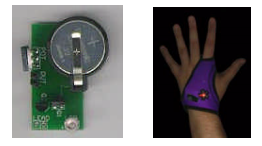
\includegraphics[scale=0.8]{img/existingdevices.png} \hspace{10mm} 
    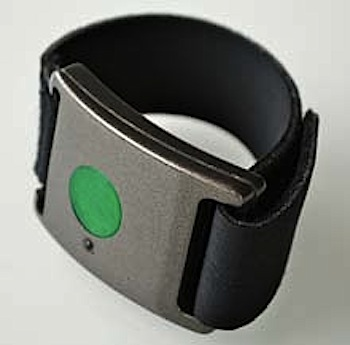
\includegraphics[scale=0.3]{img/q-sensor.jpg}\\
    The Galvactivator and Q sensor
\end{center}
\subsubsection{The Galvactivator}
The Galvactivator was created as a research exercise by Harvard. Prior to its creation,
research involving monitoring skin conductivity required electrodes to be clipped to the
experimentee's fingers. This had many drawbacks because it meant people could not be measured
whilst going about their everyday lives, and it was very difficult to acquire participants
such as children into these types of research programs. The goal of The Galvactivator was to
create a wearable skin conductivity sensor that could be worn whilst going about day to day
life. It is essentially a chip (seen on the left) with 2 small electrodes, held to the skin
by a glove (center). 

\subsubsection{Q sensor}
The technology in the Galvactivator spawned a product called the Q sensor. It was originally 
designed to measure emotional response in autistic children, this lead to a design incorporating
the galvactivator technology into a wristband, and it had to be comfortable for children. The
design also incorporates an accelerometer and a thermometer, it is also rechargable and has
bluetooth connectivity. However the Q sensor is not available for individuals to buy, and is
not designed with such thoughts in mind, it is marketed as a product for research institutions.

\subsection{Our Proposed Devices}
Our Proposed solution will require 2 devices, once will be a bracelet similar to the q sensor in
that it will contain 2 electrodes to measure skin conductivity. However the bracelet will not
contain a thermometer and accelerometer like the q sensor, thus it can be much smaller.

The second device will be on a clip which will attach to the user's lapel or dress, or anywhere
on the chest. This device will contain an accelerometer in order to measure the user's breathing
rate and depth, it will also house a small video camera which will trigger recordings at 
moments of high stress or calm.

In addition to both of these wearable devices, there will be a bowl, into which both of these
devices will be placed at the end of the day. This bowl will inductively charge the devices and
download the data from them via bluetooth. The bowl will also have wifi/3g connectivity, so once
the download from the devices is done it will upload them to the users account on the calmist
website.


TODO

\section{Giving Feedback - Personalised, Gamified Website}

\subsection{Website Concept}

We made a simple prototype of a website for our solution that would work together with a proposed device. It is an easy-to-use concept which allows the user of CALMist to see how their stress levels were changing during the day, compare different days from the past and get healthy tips in order to cope with and reduce stress. Here is a quick preview of the website:

\begin{figure}[htb]
	\begin{center}
		\fbox{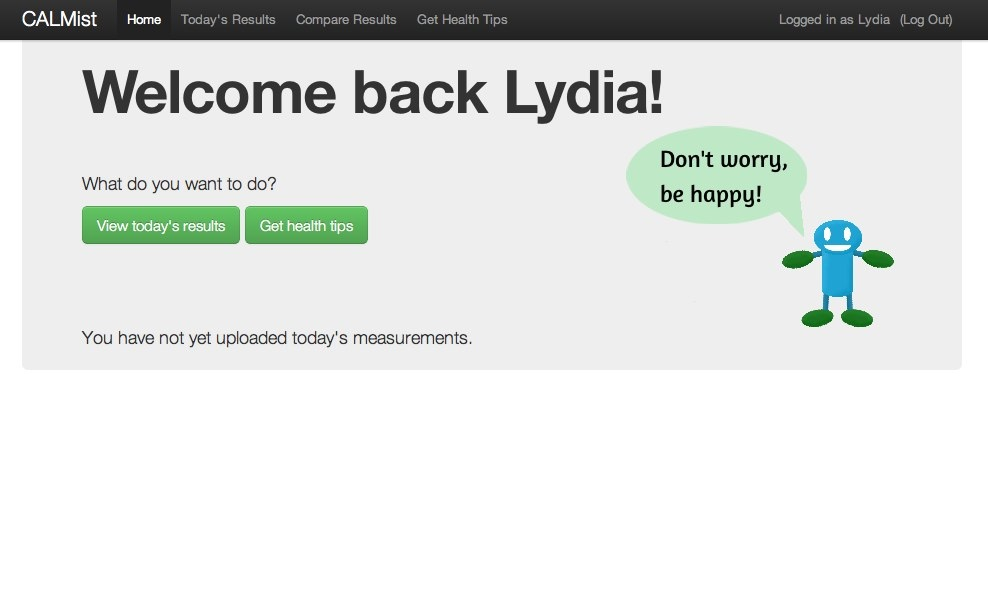
\includegraphics[scale=0.4]{index}}
    \end{center}
	\caption{Home screen}
	\label{fig:website-index}
\end{figure}

\begin{figure}[htb]
	\begin{center}
		\fbox{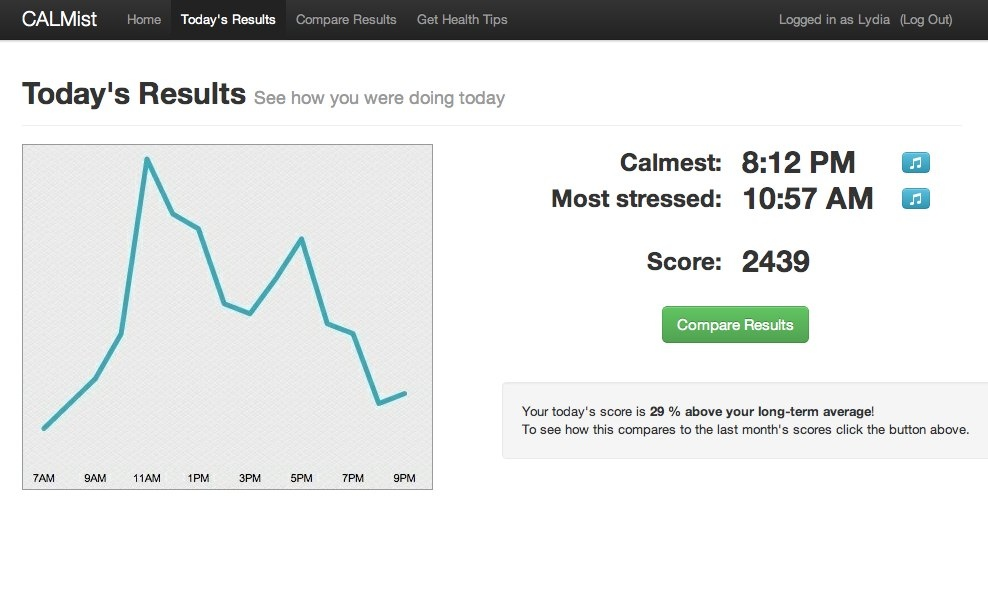
\includegraphics[scale=0.4]{todays-results}}
    \end{center}
	\caption{Screen with today's results}
	\label{fig:website-todays-results}
\end{figure}

\begin{figure}[htb]
	\begin{center}
		\fbox{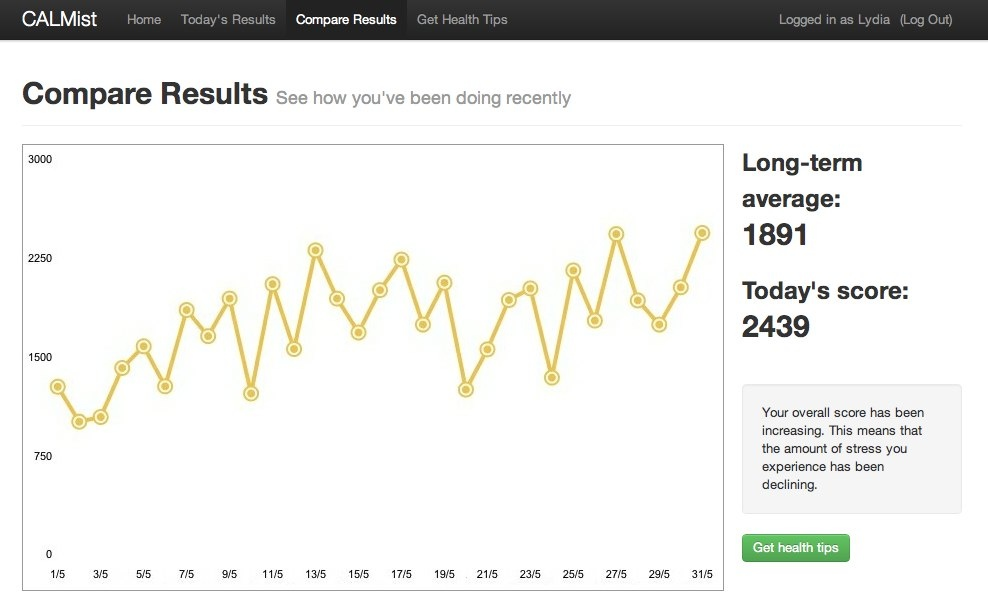
\includegraphics[scale=0.4]{compare-results}}	\end{center}
	\caption{Screen for comparing stress level scores}
	\label{fig:website-compare-results}
\end{figure}

As the home page of the website prototype (Figure ~\ref{fig:website-index}) clearly shows, emphasis is given on ease of use. The website is designed in such a way as to not stress the user.

Next, in Figure ~\ref{fig:website-todays-results}, we see a screen where the user can have a look at their stress levels throughout the day. This is shown on the left hand side while on the right hand side the website pinpoints the time when the CALMist user was calmest and most stressed on that day. Each one of these has a little icon to allow viewing a short video recording of what was going on around the user at that time. Based on the day's stress data a daily score is calculated. This might not be informative too much on its own without any further knowledge however it will allow long-term comparison of stress development.

The last screen (in Figure ~\ref{fig:website-compare-results}) shows by default a graph of stress level scores in the last month. The higher the score is the less stressed the user was. By looking at the graph the user is able to see how the amount of their stress has been changing. Scores from the whole period of time of using the CALMist are used to calculate a long-term average which allows for concluding facts like: ``Oh, I was less stressed today than usually."

Another important part of the website would inform about how to live healthy lifestyle with less stress. We do not however have a prototype for it.

\subsection{Gamification}

The website tries to encourage people to get better at managing stress using the score system. Obviously, this might not be something one can easily influence willingly. However, having users trying to beat their previous scores helps to motivate them and perhaps makes using CALMist more fun.

\section{Value Proposition}
A value proposition is the expected value to be delivered to the customer or user of the product. Essentially, it answers the
question ``why would I want this?''.

This question can be split into 4 sub-questions: What is it, who is it targeted at, why is it useful, and how is it better than
existing solutions?

\textbf{What is it?}\\
A system to help the user track their stress levels, with the aim of reducing it. Consists of discreet, wearable sensorts to collect
data without being intrusive, and a companion website to give feedback and encouragement.

\textbf{Who is it targeted at?}\\
The main target is people with stressful jobs. However, since nothing is tailored to any specific job or job category and so
is relevant in the general case, it would be useful to anybody who finds themselves under a lot of stress, or even people
who just want to make sure their levels of stress stay low!

\textbf{How is it better than existing solutions?}
It would be a push to call anything that currently exists an ``existing solution''. Hardware wise, devices do already exist that
measure stress levels, but they are not readily available to the general public. Furthermore, they are somewhat big, obvious and
intrusive. Our hardware would be readily available and unintrusive. As stated before, it is just a small chip and clip-on device.
Perhaps, worst case, it would mean you have to wear a watch when you wouldn't normally wear one, but you have the choice of what
accessory to wear. The chips are designed to be discreet and disguisable. They don't get in the way of the wearer, and they are
virtually impossible for another person to spot (which we consider the most important aspect since stress is such a personal
thing).

Software-wise, we haven't found anything similar to exist, at least not in the domain of stress management. There are plenty of
websites with tips and self-help articles, but as with our first idea they all seem rather passive. The most active website we
found was one with a game designed to try and stress you out, the objective being to stay calm. This is more of an exercise of
control rather than mangement, however, so isn't really the same thing. Our website is designed to encourage the user by 
providing positive reinforcements and helpful comments, and to let them see what is hopefully improvement over a long period of time.
If there is no improvement, we hope that it will also help the user to realise they have a serious problem and to consult a
professional about it (rather than what seems to often happen now where people make excuses or fail to notice the stress at all).

\section{Stakeholder Analysis}
The stakeholders are the people who this solution affects. This term is usually used in a business-sense, however, we feel that
a more interesting result stems from analysing this from a health point of view.

The stakeholders of this system are:

\textbf{The End Users}\\
i.e. the people who use the solution. This is for obvious reasons - the person who uses the solution is of course going to be
affected by it. Hopefully in a positive manner. The solution will record their stress levels over time and present them with
a summary and a score. The end-user then takes steps to improve their score all the while being encouraged. When their score
does improve, they have the positive reinforcement of seeing this on a simple graph, as discussed above, which will reinforce
whatever positive lifestyle changes they've made, and motivate them to keep changing things for the better.

\textbf{Employees (possibly also End Users)}\\
From an employment/work point of view, lower stress levels mean they will be less negatively affected by whatever issues they
have in the workplace. Lower stress levels also tend to mean less stress related illness and so less sick leave. While this may
not sound all that de-stressing to begin with, consider what was mentioned near the beginning of this report. More sick leave
means less time in which to do the necessary work. Businesses tend to have tight deadlines, and if you have time off you'll have
to make up for it. This means less stress due to being overworked, and less overtime (a common consequence of being overworked)
means more time for oneself to enjoy as one wishes.

\textbf{Employers}\\
Let's say their employees are very stressed, regularly taking sick leave and
are incredibly overworked. As discussed in the previous point, this solution attempts to tackle these problems. Hopefully, the
result will be lower stressed employees who take less sick leave. There are many benefits for this. Firstly, of course, less sick
leave means more usable working hours. Furthermore, lower stress levels tends to promote better morale in a person or amongst
a team of people. As such, even in the same amount of time, their employees may well become more productive. Higher productivity
is of course a key goal in management and business success.

On a more personal note, low-stress employees are less likely to
harbour feelings of resentment towards their superiors. It is often stated that being a boss (something an employer is by definition)
is very lonely (``it's lonely at the top''), because people tend to alienate you out of jealousy, work ethic or any number of
other reasons. The point is, you're in a position where you have power, but are easy to single out because of that power.
Even if people cannot directly confront you, they don't have to get on with you either. We don't make any claims regarding this,
however the solution would promote a situation where getting along with one's employees is more likely. For all of these reasons,
employers have an interest in the proposed solution.

\textbf{Doctors}\\
While the proposed solution is not a replacement for medical intervention, doctors may have an interest in the system
for a few reasons. Firstly, if the system reduces stress, they will have to deal with stress-related health issues,
which place a large strain upon health services due to the
sheer number of cases.
Of course, some unscrupulous private health companies may not consider less patients a
good thing, even if due to better general health. However, ignoring the politics of the matter, this can only be taken as a positive.
Also, if the system encorages people whom have serious stress-related issues
to see a professional, a greater proportion of the patients doctors see for stress-related issues may be relevant. People
often go to see a doctor when a simple lifestyle change may help them and/or where they
simply do not realise the issue is stress. This in theory will help the treatment doctors give to be as effective as possible, as
less time will be wasted on people who don't really need medical intervention so that all effort can be focused on those who do.

Furthermore, diagnosing stress-related disorders is often a very difficult and inexact process, very often involving the doctor
asking the patient to keep a ``Stress Diary'' for about 2 weeks. This 
delays any diagnosis and treatment.
Also, although stress is a subjective topic anyway, it is bad that diaries are also subjective. it is very difficult to
quantify the information they contain. This is where the proposed solution could potentially help.
Firstly, the user will already have a log of their stress
levels, and secondly, the data in the log is from actual
measurements. It is impractical for a doctor to ask a patient to walk around with electrodes stuck to them for a couple of weeks,
so they must rely on essentially unquantifiable data from a diary. However, the system succeeds in quantifying more or less what
the diary is trying to measure. Going by this data may well be far less ambigous, and lead to a faster and
more accurate diagnosis. Again, while we make no medical claims for the solution, we wouldn't be surprised if, once produced,
it were to be recommended by health professionals in some shape or form. We don't see it as impossible that it could replace
the stress diary altogether, although that's a bold claim and not one we would make so frivilously. As such, doctors may
well have an interest in the proposed solution.

\section{Appendix - Questionnaires}
Here are a few of the sample responses we got from our questionaires:
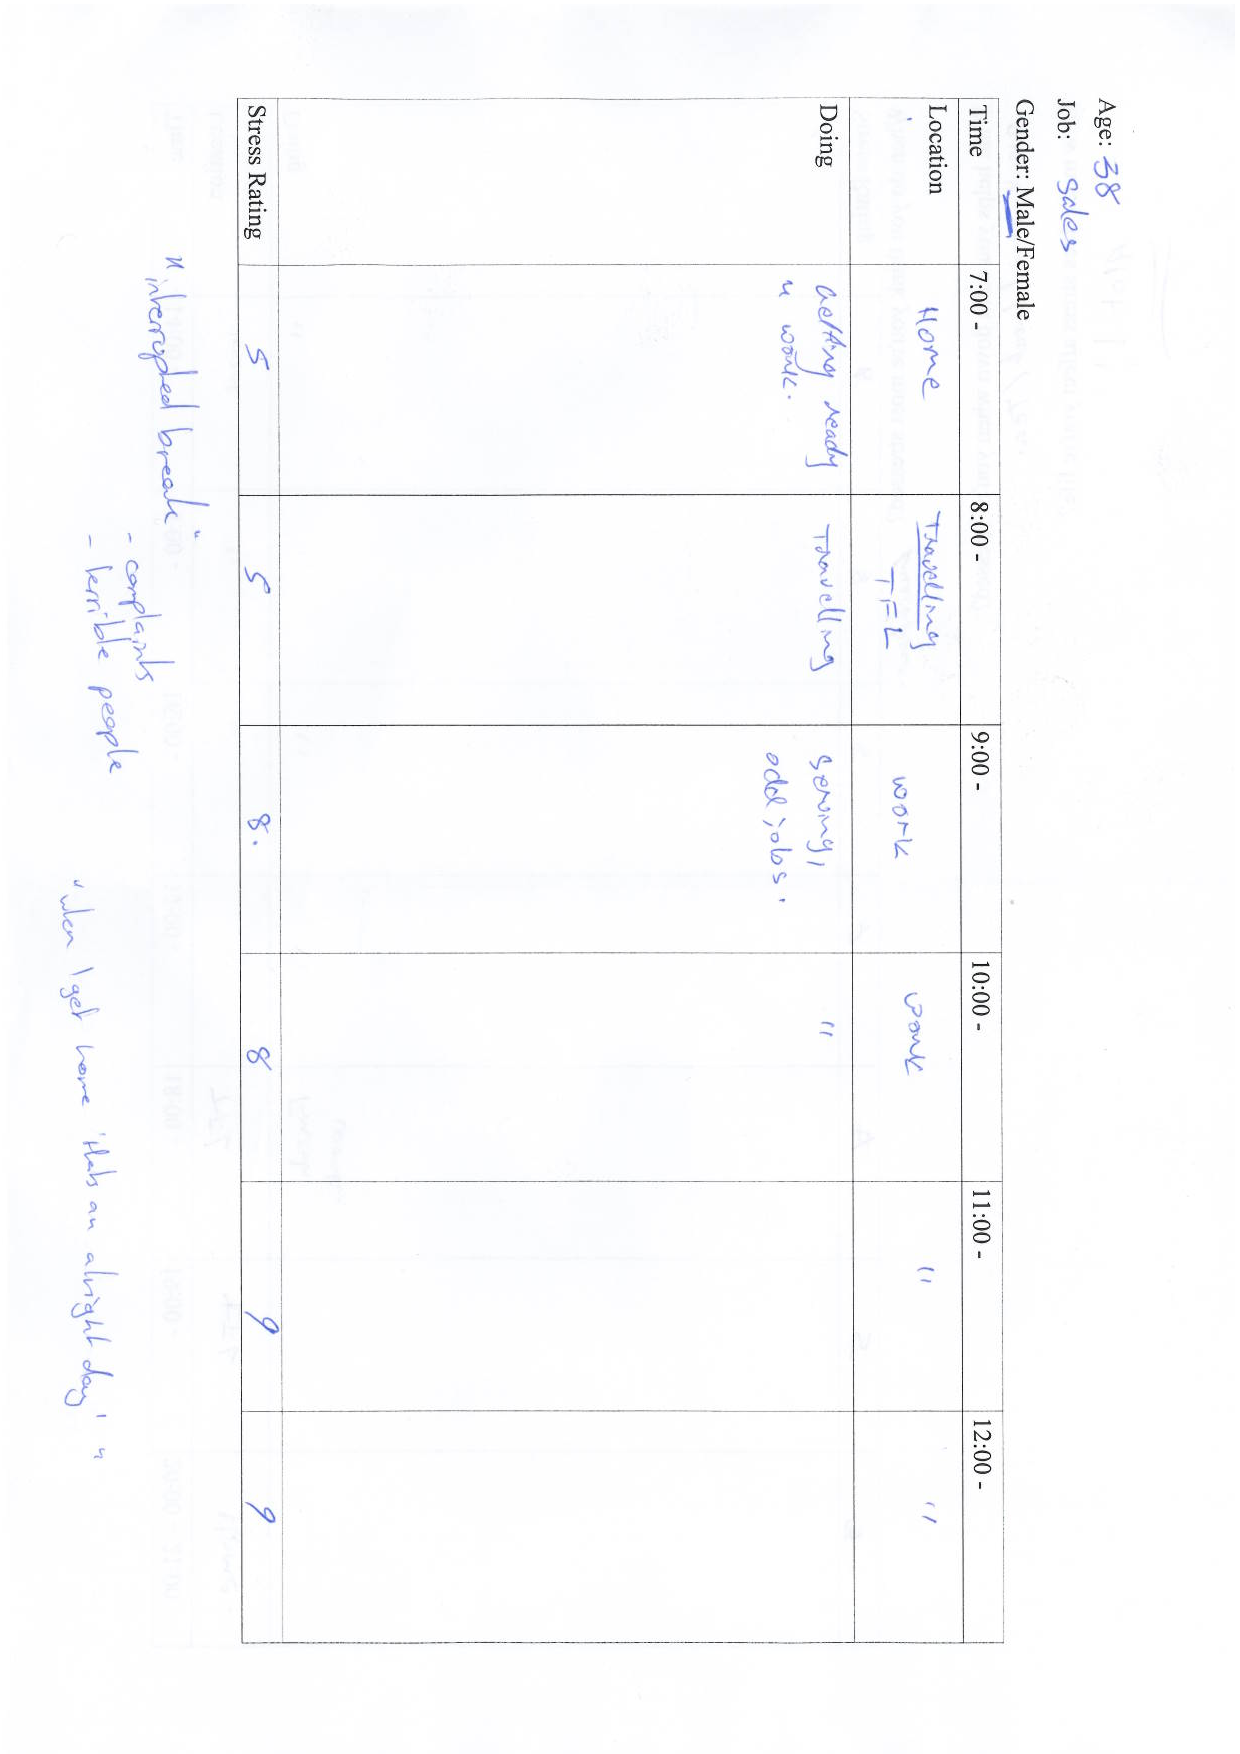
\includepdf{PDFResponses/Ryman1}
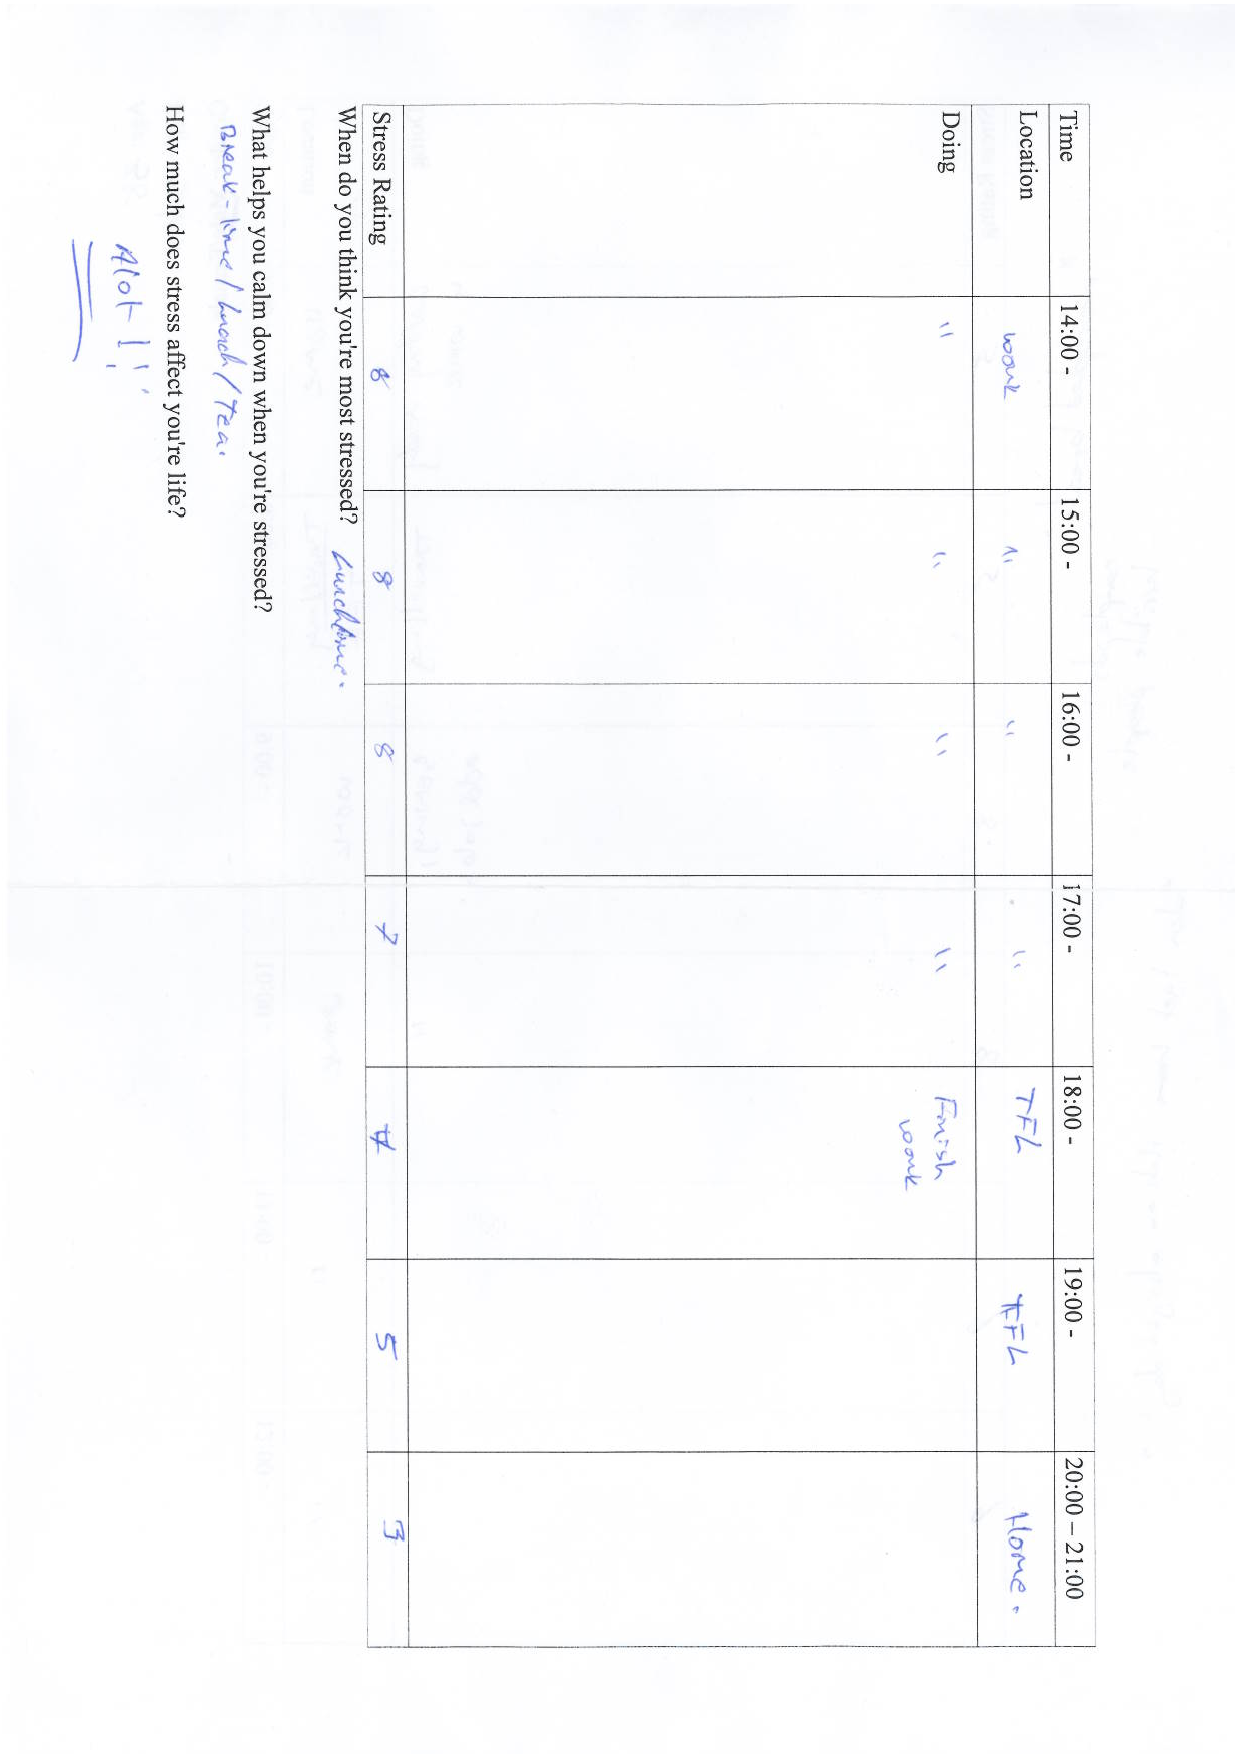
\includepdf{PDFResponses/Ryman2}
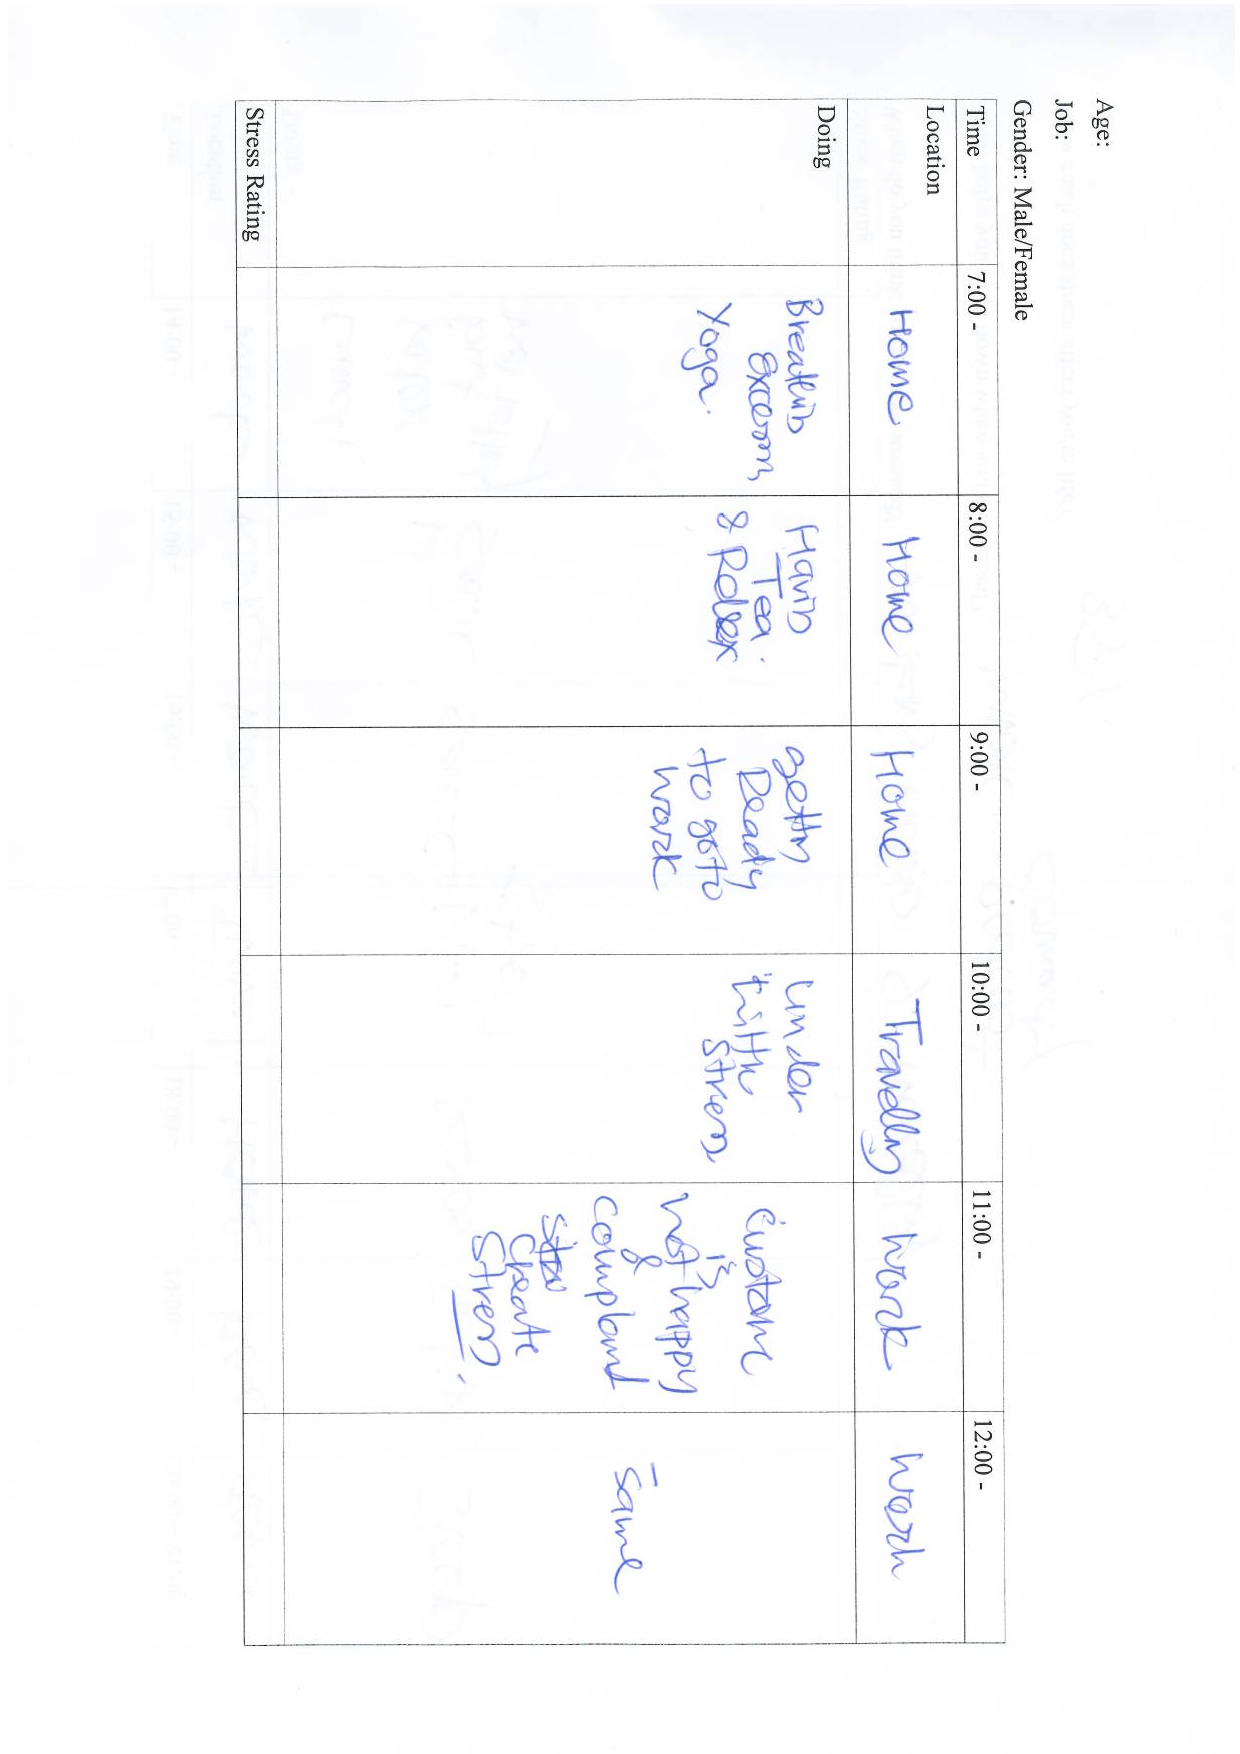
\includepdf{PDFResponses/Kodak1}
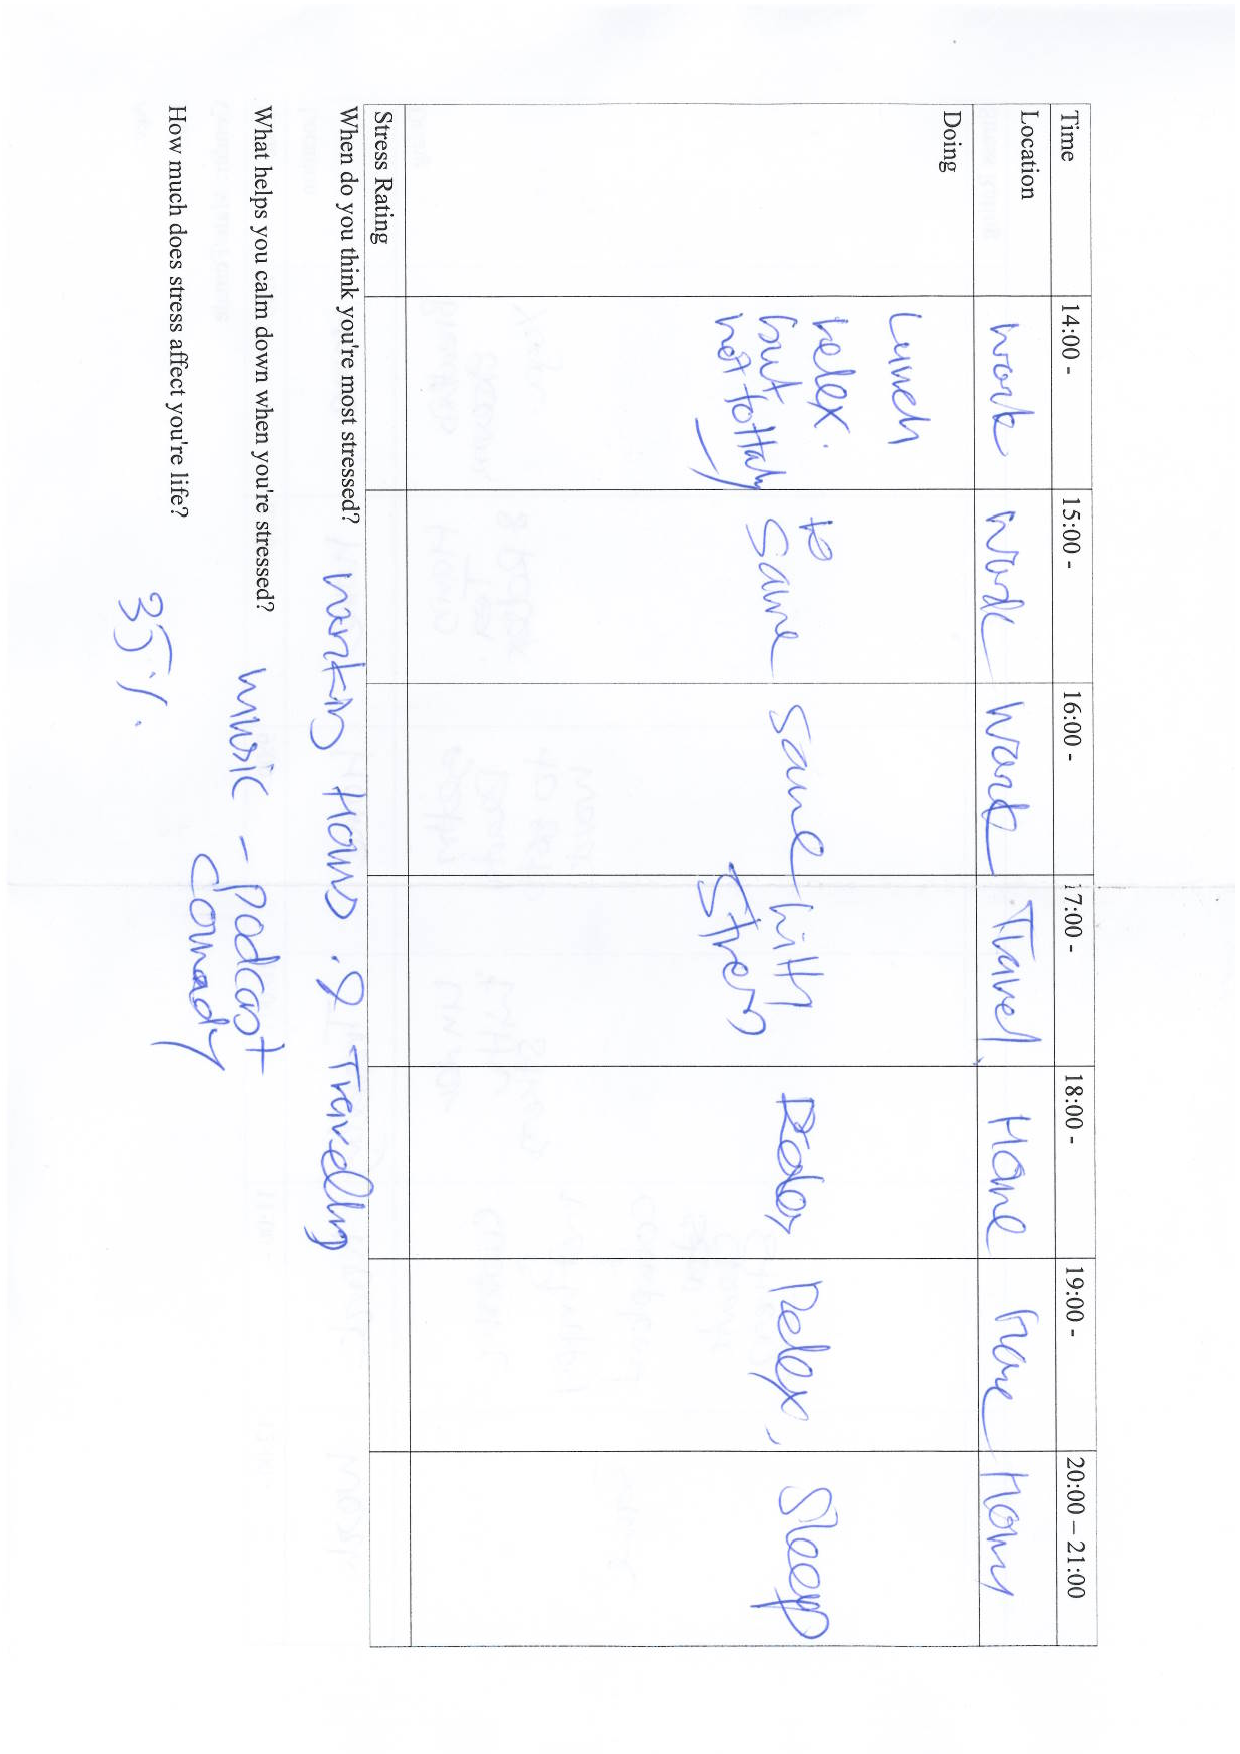
\includepdf{PDFResponses/Kodak2}
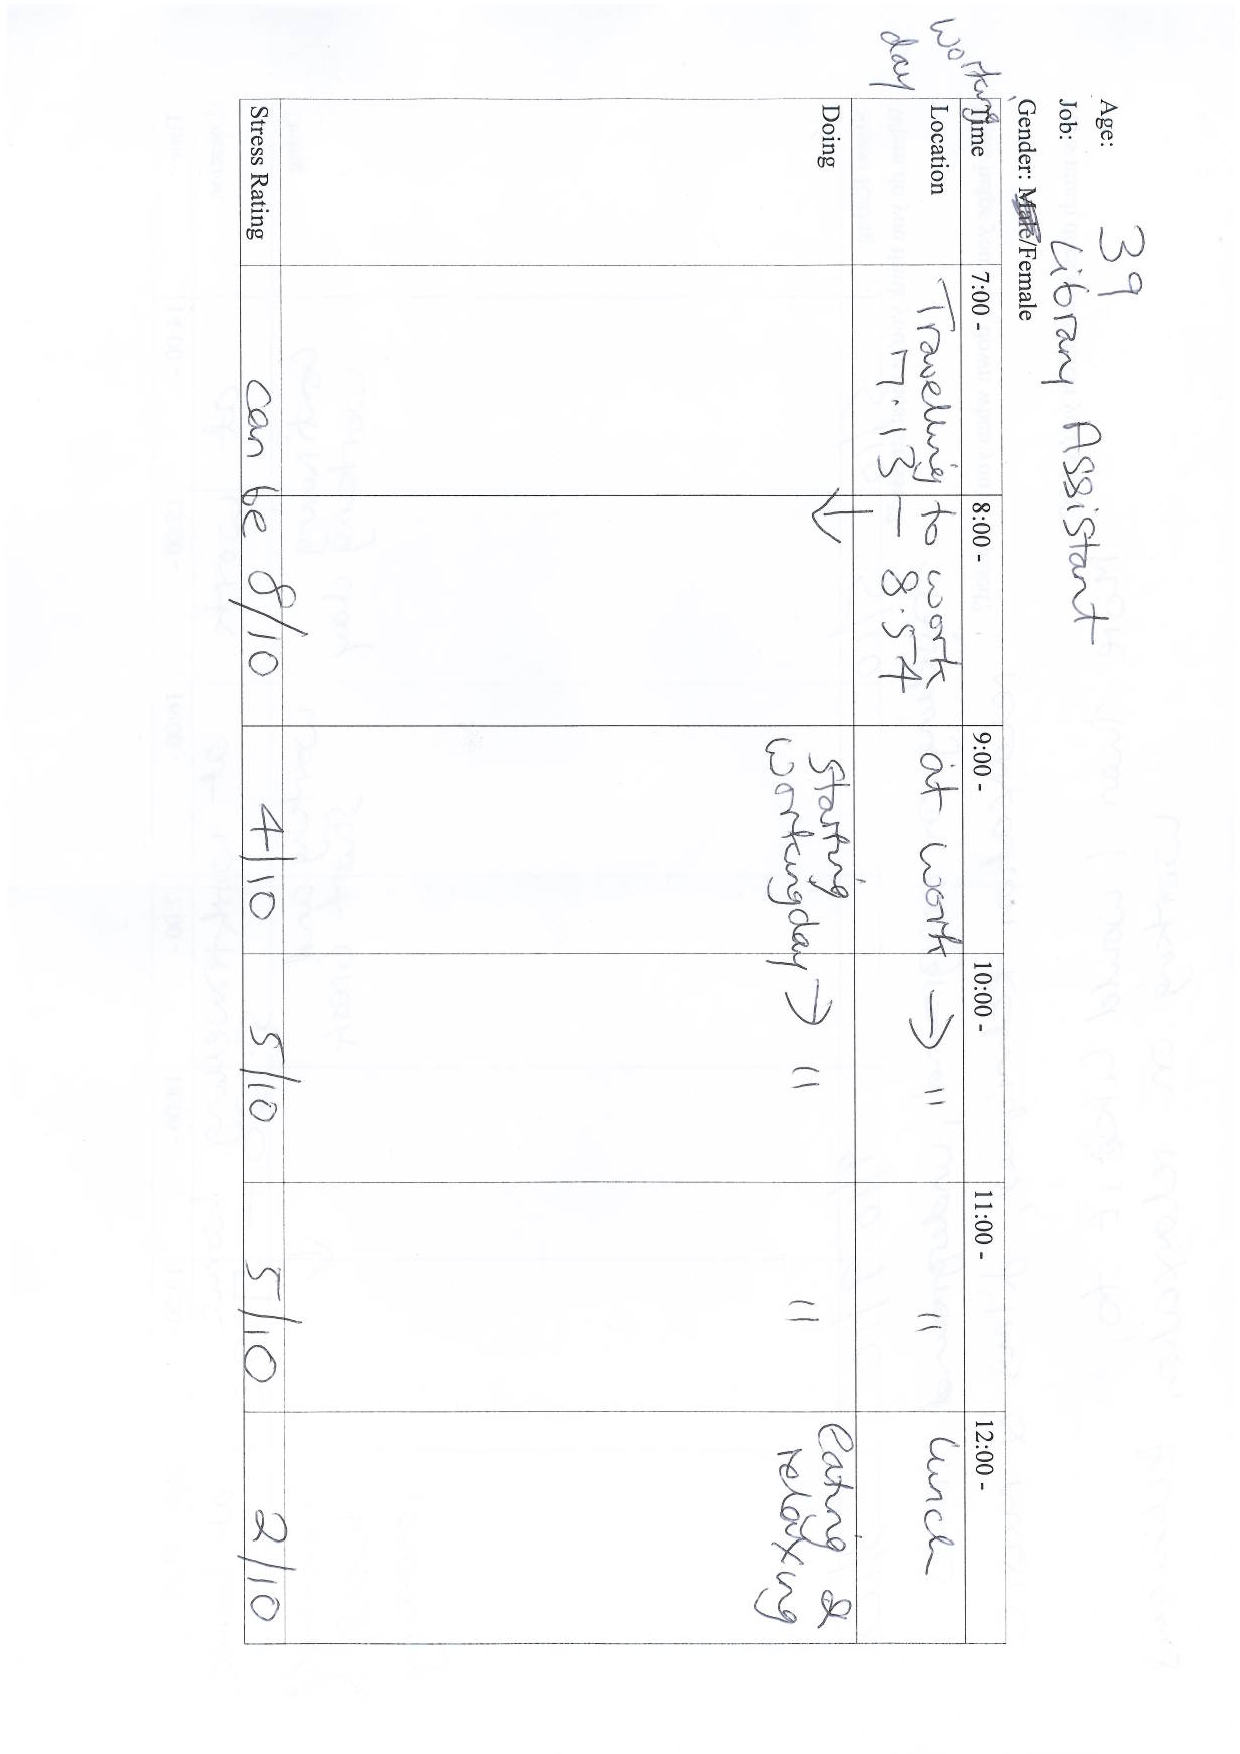
\includepdf{PDFResponses/LibraryAssistant1}
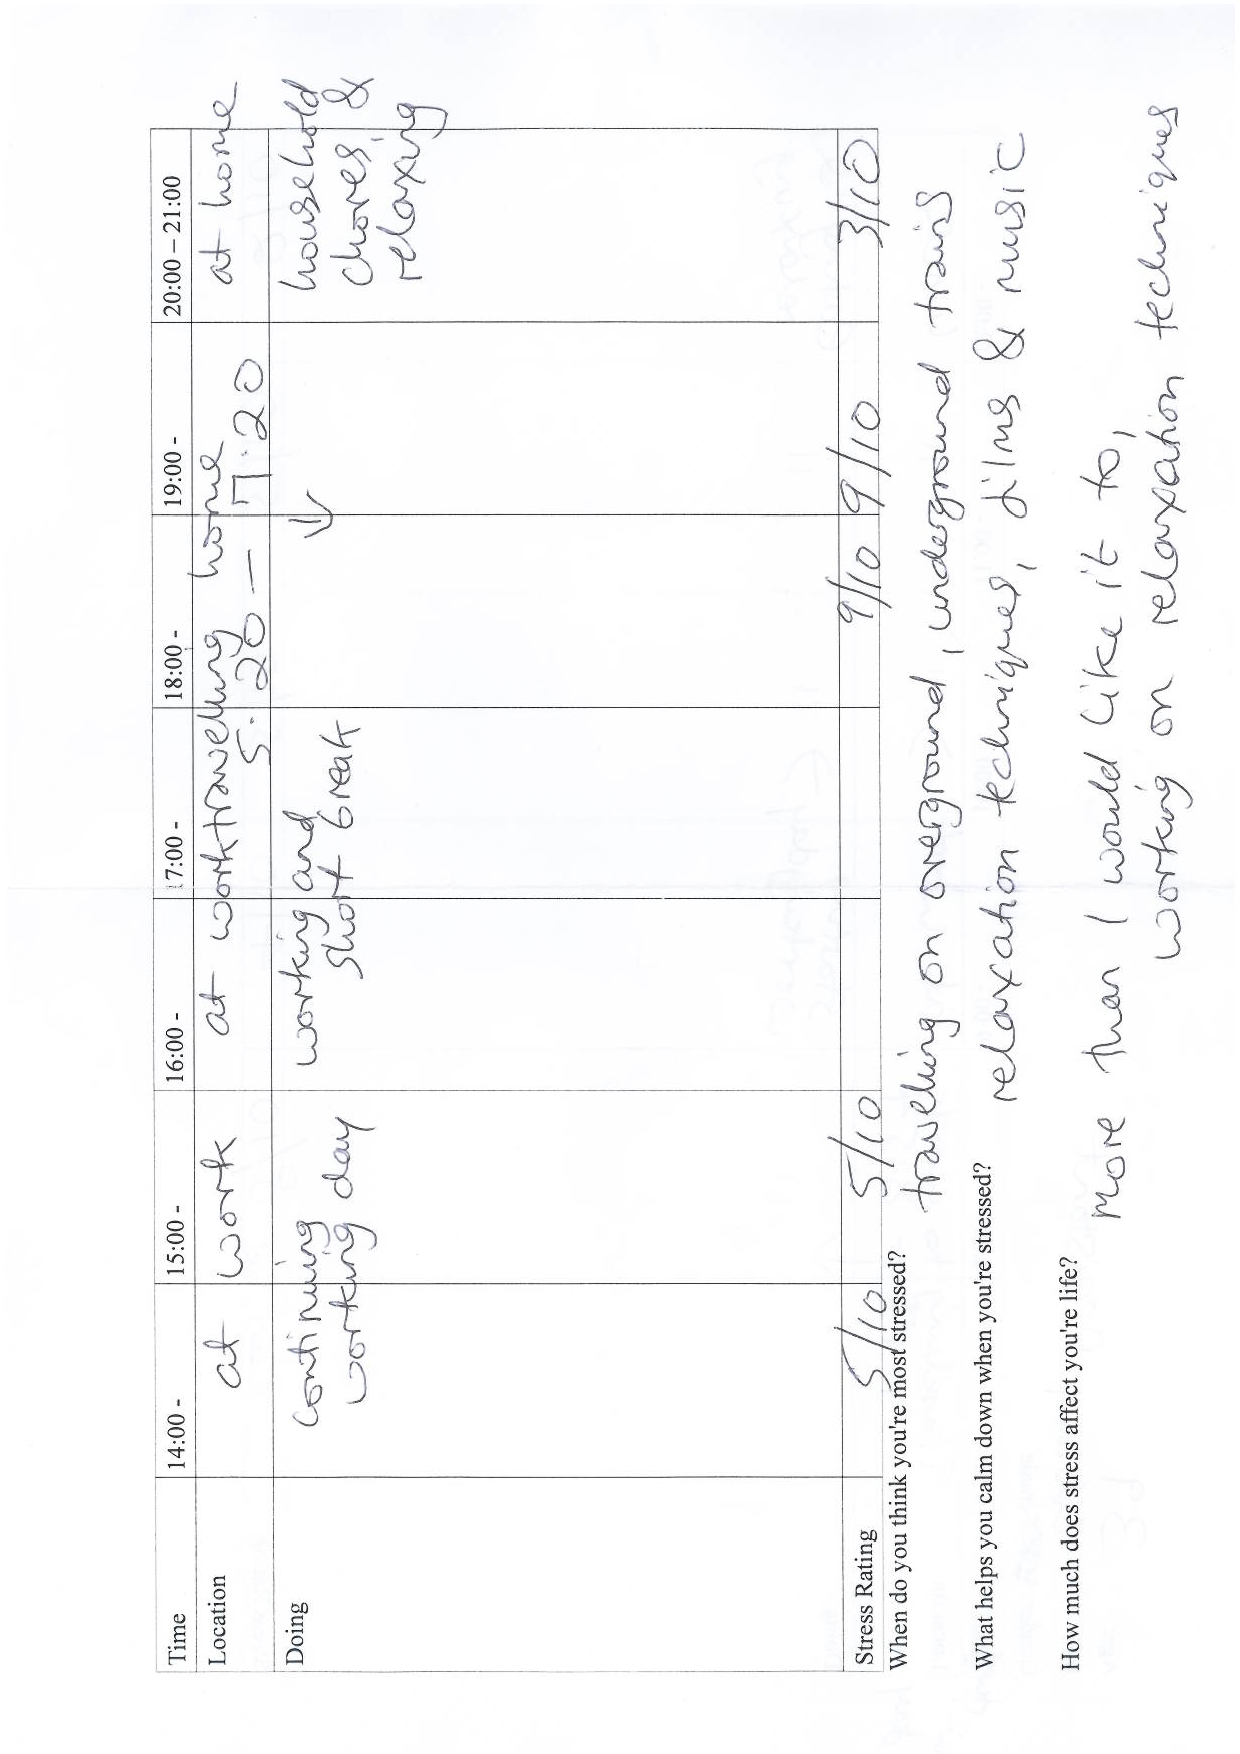
\includepdf[angle=180]{PDFResponses/LibraryAssistant2}
\end{document}
